\markdownRendererDocumentBegin
\markdownRendererWarning{The `hybrid` option has been soft-deprecated.}{The `hybrid` option has been soft-deprecated.}{Consider using one of the following better options for mixing TeX and markdown: `contentBlocks`, `rawAttribute`, `texComments`, `texMathDollars`, `texMathSingleBackslash`, and `texMathDoubleBackslash`. For more information, see the user manual at <https://witiko.github.io/markdown/>.}{Consider using one of the following better options for mixing TeX and markdown: `contentBlocks`, `rawAttribute`, `texComments`, `texMathDollars`, `texMathSingleBackslash`, and `texMathDoubleBackslash`. For more information, see the user manual at <https://witiko.github.io/markdown/>.}This script uses OpenCV and EasyOCR to capture video from a webcam, identify and read text from two specific regions (voltage and temperature in this case), and log this data to a file.\markdownRendererParagraphSeparator
{}It is designed to be calibrated for a specific, fixed-camera setup, such as this case where we are reading data from an LCD screen and a separate standard thermometer.\markdownRendererInterblockSeparator
{}\markdownRendererSectionBegin
\markdownRendererSectionBegin
\markdownRendererHeadingTwo{\markdownRendererStrongEmphasis{Getting Started}}\markdownRendererInterblockSeparator
{}Follow these instructions to get the script up and running on your local machine.\markdownRendererInterblockSeparator
{}\markdownRendererSectionBegin
\markdownRendererHeadingThree{\markdownRendererStrongEmphasis{Prerequisites}}\markdownRendererInterblockSeparator
{}Before you run the script, you'll need a few things set up.\markdownRendererParagraphSeparator
{}\markdownRendererStrongEmphasis{Hardware:}\markdownRendererInterblockSeparator
{}\markdownRendererUlBeginTight
\markdownRendererUlItem A webcam connected to your computer.\markdownRendererUlItemEnd 
\markdownRendererUlItem \markdownRendererStrongEmphasis{(Not necessary)} An NVIDIA GPU with CUDA installed. The script is pre-set to use \markdownRendererCodeSpan{gpu=True} for much faster processing.\markdownRendererUlItemEnd 
\markdownRendererUlEndTight \markdownRendererInterblockSeparator
{}\markdownRendererStrongEmphasis{Software:}\markdownRendererInterblockSeparator
{}\markdownRendererUlBeginTight
\markdownRendererUlItem Python 3.x\markdownRendererUlItemEnd 
\markdownRendererUlItem The required Python libraries:  \markdownRendererCodeSpan{opencv-python}\markdownRendererCite{1}+{}{}{opencv}, \markdownRendererCodeSpan{easyocr}\markdownRendererCite{1}+{}{}{easyocr}, and \markdownRendererCodeSpan{numpy}\markdownRendererCite{1}+{}{}{numpy}.\markdownRendererUlItemEnd 
\markdownRendererUlEndTight \markdownRendererInterblockSeparator
{}
\markdownRendererSectionEnd \markdownRendererSectionBegin
\markdownRendererHeadingThree{\markdownRendererStrongEmphasis{A Note on the Webcam (Optional)}}\markdownRendererInterblockSeparator
{}This script will work with any webcam that OpenCV can detect, including built-in laptop cameras or standard USB webcams. The most important factor is a stable, well-positioned camera.\markdownRendererParagraphSeparator
{}For reference, the development and testing for this project were done using a virtual camera setup:\markdownRendererInterblockSeparator
{}\markdownRendererUlBegin
\markdownRendererUlItem DroidCam\markdownRendererCite{1}+{}{}{droidcam}: An application to use a smartphone as a high-quality webcam.\markdownRendererUlItemEnd 
\markdownRendererUlItem OBS Studio\markdownRendererCite{1}+{}{}{obsstudio}: This software was used to capture the DroidCam feed and output it as an "OBS Virtual Camera," which was then selected by the Python script.\markdownRendererUlItemEnd 
\markdownRendererUlEnd \markdownRendererInterblockSeparator
{}Again, this specific setup is not required. It is just one example of how to provide a camera feed to the script. Any simple webcam will work perfectly fine.\markdownRendererInterblockSeparator
{}
\markdownRendererSectionEnd \markdownRendererSectionBegin
\markdownRendererHeadingThree{\markdownRendererStrongEmphasis{Installation}}\markdownRendererInterblockSeparator
{}\markdownRendererUlBegin
\markdownRendererUlItem \markdownRendererStrongEmphasis{Create a Directory for Images:}\markdownRendererSoftLineBreak
{}The script is hardcoded to save debug images to an \markdownRendererCodeSpan{img/} folder. You must create this folder in the same directory as the script for the program to run.\markdownRendererInterblockSeparator
{}\markdownRendererInputFencedCode{./_markdown_main/acc8ab3565abbcc7491c2d9aeb1de99d.verbatim}{bash}{bash}\markdownRendererUlItemEnd 
\markdownRendererUlItem \markdownRendererStrongEmphasis{Install Python Libraries:}\markdownRendererSoftLineBreak
{}Install the necessary packages using \markdownRendererCodeSpan{pip}:\markdownRendererInterblockSeparator
{}\markdownRendererInputFencedCode{./_markdown_main/9362dfb488eea26e057a3e07b89e9a27.verbatim}{bash}{bash}\markdownRendererInterblockSeparator
{}\markdownRendererBlockQuoteBegin
\markdownRendererStrongEmphasis{Note:} easyocr\markdownRendererCite{1}+{}{}{easyocr} will also install PyTorch\markdownRendererCite{1}+{}{}{pytorch}, which is a large download and a required dependency.\markdownRendererBlockQuoteEnd \markdownRendererUlItemEnd 
\markdownRendererUlEnd \markdownRendererInterblockSeparator
{}
\markdownRendererSectionEnd 
\markdownRendererSectionEnd \markdownRendererSectionBegin
\markdownRendererHeadingTwo{\markdownRendererStrongEmphasis{How to Run}}\markdownRendererInterblockSeparator
{}\markdownRendererOlBeginTight
\markdownRendererOlItemWithNumber{1}Make sure your webcam is plugged in and positioned correctly to see both your target readings.\markdownRendererOlItemEnd 
\markdownRendererOlItemWithNumber{2}Open a terminal and navigate to the folder containing \markdownRendererCodeSpan{a.py}.\markdownRendererOlItemEnd 
\markdownRendererOlItemWithNumber{3}Run the script:\markdownRendererInterblockSeparator
{}\markdownRendererInputFencedCode{./_markdown_main/6bde01e7a8c90d081242bec0d64b1aa6.verbatim}{bash}{bash}\markdownRendererOlItemEnd 
\markdownRendererOlItemWithNumber{4}Two windows will appear: 'Voltage' and 'Temperature'. These show the exact (and processed) regions being sent to the OCR engine.\markdownRendererOlItemEnd 
\markdownRendererOlItemWithNumber{5}To stop the script, make sure one of these windows is active (click on it) and \markdownRendererStrongEmphasis{press the 'q' key}.\markdownRendererOlItemEnd 
\markdownRendererOlEndTight \markdownRendererParagraphSeparator
{}
\markdownRendererSectionEnd \markdownRendererSectionBegin
\markdownRendererHeadingTwo{\markdownRendererStrongEmphasis{Important: Calibration is Required!}}\markdownRendererInterblockSeparator
{}This script \markdownRendererStrongEmphasis{will not work correctly} without calibration. You must adjust the code to fit your specific camera, lighting, and display setup.\markdownRendererParagraphSeparator
{}Here are the key sections you \markdownRendererStrongEmphasis{must} modify in \markdownRendererCodeSpan{a.py}:\markdownRendererInterblockSeparator
{}\markdownRendererSectionBegin
\markdownRendererHeadingThree{\markdownRendererStrongEmphasis{GPU Usage}}\markdownRendererInterblockSeparator
{}If you \markdownRendererStrongEmphasis{do not} have a compatible NVIDIA GPU, you must change this line:\markdownRendererInterblockSeparator
{}\markdownRendererInputFencedCode{./_markdown_main/e53b762886c61029f075343677220dc0.verbatim}{python}{python}\markdownRendererInterblockSeparator
{}The script will run much slower on the CPU but will still function.\markdownRendererInterblockSeparator
{}
\markdownRendererSectionEnd \markdownRendererSectionBegin
\markdownRendererHeadingThree{\markdownRendererStrongEmphasis{Frame Cropping}}\markdownRendererInterblockSeparator
{}This is the most critical part. You need to tell the script exactly where to look for your data.\markdownRendererInterblockSeparator
{}\markdownRendererInputFencedCode{./_markdown_main/a9868d2b1a186e78de5810120a2daa9d.verbatim}{python}{python}\markdownRendererInterblockSeparator
{}Python slices are in [y1:y2, x1:x2] format (rows, then columns).\markdownRendererParagraphSeparator
{}\markdownRendererCodeSpan{voltage\markdownRendererUnderscore{}frame} is currently set to the top half of the entire camera feed.\markdownRendererParagraphSeparator
{}\markdownRendererCodeSpan{temp\markdownRendererUnderscore{}frame} is set to the bottom-left third of the feed.\markdownRendererParagraphSeparator
{}You must change these pixel/percentage values to precisely isolate your voltage and temperature readings. The \markdownRendererCodeSpan{Voltage} and \markdownRendererCodeSpan{Temperature} windows will show you what the script sees in these cropped zones, so you can adjust the values and re-run until they are correct.\markdownRendererInterblockSeparator
{}
\markdownRendererSectionEnd \markdownRendererSectionBegin
\markdownRendererHeadingThree{\markdownRendererStrongEmphasis{Image Processing}}\markdownRendererInterblockSeparator
{}\markdownRendererUlBeginTight
\markdownRendererUlItem \markdownRendererStrongEmphasis{Temperature}\markdownRendererUlItemEnd 
\markdownRendererUlEndTight \markdownRendererInterblockSeparator
{}\markdownRendererInputFencedCode{./_markdown_main/c191fdafa67f206e9c26c489e01b63be.verbatim}{python}{python}\markdownRendererInterblockSeparator
{}\markdownRendererSectionBegin
\markdownRendererSectionBegin
\markdownRendererHeadingFive{Key Values to Change:}\markdownRendererInterblockSeparator
{}\markdownRendererUlBegin
\markdownRendererUlItem \markdownRendererCodeSpan{cv2.threshold(gray\markdownRendererUnderscore{}t,130, 255, cv2.THRESH\markdownRendererUnderscore{}BINARY\markdownRendererUnderscore{}INV)}: The 130 is the threshold value. This is highly sensitive to lighting. Adjust it up or down until the text is clearly separated from the background in the 'Temperature' window.\markdownRendererUlItemEnd 
\markdownRendererUlItem \markdownRendererCodeSpan{cv2.getStructuringElement(cv2.MORPH\markdownRendererUnderscore{}RECT, (11,11))}: This is the kernel size for the 'closing' operation, which helps connect broken parts of a number. You may need to make it larger or smaller.\markdownRendererUlItemEnd 
\markdownRendererUlItem \markdownRendererCodeSpan{cv2.GaussianBlur(pretemp, (17,17), 0)}: This is the kernel size for the blur.\markdownRendererUlItemEnd 
\markdownRendererUlEnd \markdownRendererInterblockSeparator
{}Look at the \markdownRendererCodeSpan{Temperature} window while calibrating. Your goal is to make the numbers you want to read clear and solid, while removing as much background noise as possible.\markdownRendererParagraphSeparator
{}It is also preferred to hide the decimal point, either physically or by further image processing.\markdownRendererInterblockSeparator
{}\markdownRendererUlBeginTight
\markdownRendererUlItem \markdownRendererStrongEmphasis{Voltage}\markdownRendererSoftLineBreak
{}In this case, the cropped voltage frame, is converted to grayscale before it is used for OCR. Make sure the voltage reading is visible in the voltage frame. It is also preferred to hide the decimal point, either physically or by further image processing.\markdownRendererUlItemEnd 
\markdownRendererUlEndTight \markdownRendererInterblockSeparator
{}
\markdownRendererSectionEnd 
\markdownRendererSectionEnd 
\markdownRendererSectionEnd 
\markdownRendererSectionEnd \markdownRendererSectionBegin
\markdownRendererHeadingTwo{\markdownRendererStrongEmphasis{Data Collection Methodology}}\markdownRendererInterblockSeparator
{}The dataset is collected by simulating a \markdownRendererStrongEmphasis{real-world thermal change (cooling cycle)} to capture paired temperature readings.\markdownRendererParagraphSeparator
{}\begin{figure}[h!]\markdownRendererSoftLineBreak
{}\centering\markdownRendererSoftLineBreak
{}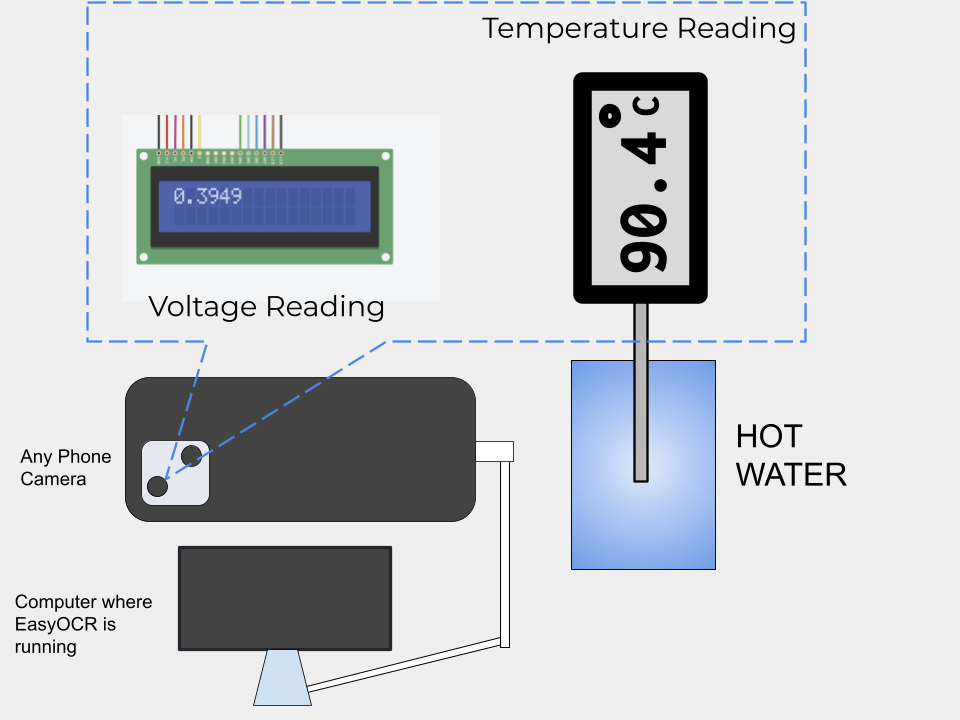
\includegraphics[width=0.8\linewidth]{figs/autotrainer_schematic.png}\markdownRendererSoftLineBreak
{}\caption{Auto-Trainer representation}\markdownRendererSoftLineBreak
{}\label{fig:autotrainer_schematic}\markdownRendererSoftLineBreak
{}\end{figure}\markdownRendererInterblockSeparator
{}\markdownRendererOlBegin
\markdownRendererOlItemWithNumber{1}\markdownRendererStrongEmphasis{Setup:}\markdownRendererInterblockSeparator
{}\markdownRendererUlBeginTight
\markdownRendererUlItem Place both the PT100 probe and the reference thermometer inside an electric kettle, submerged in water.\markdownRendererUlItemEnd 
\markdownRendererUlEndTight \markdownRendererOlItemEnd 
\markdownRendererOlItemWithNumber{2}\markdownRendererStrongEmphasis{Heating Phase:}\markdownRendererInterblockSeparator
{}\markdownRendererUlBeginTight
\markdownRendererUlItem Turn on the kettle and heat the water to its boiling point.\markdownRendererUlItemEnd 
\markdownRendererUlEndTight \markdownRendererOlItemEnd 
\markdownRendererOlItemWithNumber{3}\markdownRendererStrongEmphasis{Recording Phase:}\markdownRendererInterblockSeparator
{}\markdownRendererUlBeginTight
\markdownRendererUlItem Switch off the kettle at boiling point.\markdownRendererUlItemEnd 
\markdownRendererUlItem Start recording a \markdownRendererStrongEmphasis{video} using the smartphone.\markdownRendererUlItemEnd 
\markdownRendererUlItem Ensure \markdownRendererStrongEmphasis{both the PT100 LCD display} and \markdownRendererStrongEmphasis{reference thermometer} are visible in the frame.\markdownRendererUlItemEnd 
\markdownRendererUlEndTight \markdownRendererOlItemEnd 
\markdownRendererOlItemWithNumber{4}\markdownRendererStrongEmphasis{Cooling Phase:}\markdownRendererInterblockSeparator
{}\markdownRendererUlBeginTight
\markdownRendererUlItem Continue recording the cooling process as the water temperature drops naturally.\markdownRendererUlItemEnd 
\markdownRendererUlEndTight \markdownRendererOlItemEnd 
\markdownRendererOlItemWithNumber{5}\markdownRendererStrongEmphasis{Data Extraction:}\markdownRendererInterblockSeparator
{}\markdownRendererUlBeginTight
\markdownRendererUlItem The recorded video acts as the raw dataset.\markdownRendererUlItemEnd 
\markdownRendererUlItem Extract frames and apply \markdownRendererStrongEmphasis{OCR (Optical Character Recognition)} to detect readings from both displays.\markdownRendererUlItemEnd 
\markdownRendererUlEndTight \markdownRendererOlItemEnd 
\markdownRendererOlEnd \markdownRendererParagraphSeparator
{}
\markdownRendererSectionEnd \markdownRendererSectionBegin
\markdownRendererHeadingTwo{\markdownRendererStrongEmphasis{Output}}\markdownRendererInterblockSeparator
{}The script generates two types of output:\markdownRendererInterblockSeparator
{}\markdownRendererUlBegin
\markdownRendererUlItem \markdownRendererCodeSpan{out.txt}: A text file that logs the detected readings. Every 15 frames, if text is found in both regions, a new line is added, formatted as: \markdownRendererCodeSpan{[voltage\markdownRendererUnderscore{}reading] [temperature\markdownRendererUnderscore{}reading]}\markdownRendererUlItemEnd 
\markdownRendererUlItem \markdownRendererCodeSpan{img/} Directory: This folder saves voltageXX.png and tempXX.png images. These are the exact frames that were sent to EasyOCR. If you are getting bad readings, check these images to see why. They are perfect for debugging your calibration and fixing the readings.\markdownRendererUlItemEnd 
\markdownRendererUlEnd \markdownRendererInterblockSeparator
{}\markdownRendererCodeSpan{out.txt} is not perfect due to some instances of incorrect character recognition. The data was manually updated and is saved in \markdownRendererCodeSpan{trainingdata.txt}
\markdownRendererSectionEnd 
\markdownRendererSectionEnd \markdownRendererDocumentEnd